\documentclass[12pt,]{article}
\usepackage{lmodern}
\usepackage{amssymb,amsmath}
\usepackage{ifxetex,ifluatex}
\usepackage{fixltx2e} % provides \textsubscript
\ifnum 0\ifxetex 1\fi\ifluatex 1\fi=0 % if pdftex
  \usepackage[T1]{fontenc}
  \usepackage[utf8]{inputenc}
\else % if luatex or xelatex
  \ifxetex
    \usepackage{mathspec}
  \else
    \usepackage{fontspec}
  \fi
  \defaultfontfeatures{Ligatures=TeX,Scale=MatchLowercase}
\fi
% use upquote if available, for straight quotes in verbatim environments
\IfFileExists{upquote.sty}{\usepackage{upquote}}{}
% use microtype if available
\IfFileExists{microtype.sty}{%
\usepackage{microtype}
\UseMicrotypeSet[protrusion]{basicmath} % disable protrusion for tt fonts
}{}
\usepackage[left=1in,right=1in,top=1in,bottom=1in]{geometry}
\usepackage{hyperref}
\hypersetup{unicode=true,
            pdfborder={0 0 0},
            breaklinks=true}
\urlstyle{same}  % don't use monospace font for urls
\usepackage{graphicx,grffile}
\makeatletter
\def\maxwidth{\ifdim\Gin@nat@width>\linewidth\linewidth\else\Gin@nat@width\fi}
\def\maxheight{\ifdim\Gin@nat@height>\textheight\textheight\else\Gin@nat@height\fi}
\makeatother
% Scale images if necessary, so that they will not overflow the page
% margins by default, and it is still possible to overwrite the defaults
% using explicit options in \includegraphics[width, height, ...]{}
\setkeys{Gin}{width=\maxwidth,height=\maxheight,keepaspectratio}
\IfFileExists{parskip.sty}{%
\usepackage{parskip}
}{% else
\setlength{\parindent}{0pt}
\setlength{\parskip}{6pt plus 2pt minus 1pt}
}
\setlength{\emergencystretch}{3em}  % prevent overfull lines
\providecommand{\tightlist}{%
  \setlength{\itemsep}{0pt}\setlength{\parskip}{0pt}}
\setcounter{secnumdepth}{5}
% Redefines (sub)paragraphs to behave more like sections
\ifx\paragraph\undefined\else
\let\oldparagraph\paragraph
\renewcommand{\paragraph}[1]{\oldparagraph{#1}\mbox{}}
\fi
\ifx\subparagraph\undefined\else
\let\oldsubparagraph\subparagraph
\renewcommand{\subparagraph}[1]{\oldsubparagraph{#1}\mbox{}}
\fi

%%% Use protect on footnotes to avoid problems with footnotes in titles
\let\rmarkdownfootnote\footnote%
\def\footnote{\protect\rmarkdownfootnote}

%%% Change title format to be more compact
\usepackage{titling}

% Create subtitle command for use in maketitle
\newcommand{\subtitle}[1]{
  \posttitle{
    \begin{center}\large#1\end{center}
    }
}

\setlength{\droptitle}{-2em}

  \title{}
    \pretitle{\vspace{\droptitle}}
  \posttitle{}
    \author{}
    \preauthor{}\postauthor{}
    \date{}
    \predate{}\postdate{}
  
\usepackage{booktabs}
\usepackage{longtable}
\usepackage{array}
\usepackage{multirow}
\usepackage[table]{xcolor}
\usepackage{wrapfig}
\usepackage{float}
\usepackage{colortbl}
\usepackage{pdflscape}
\usepackage{tabu}
\usepackage{threeparttable}
\usepackage{threeparttablex}
\usepackage[normalem]{ulem}
\usepackage{makecell}

\setlength{\parindent}{2em}
\setlength{\parskip}{0em}
\usepackage{placeins}
\usepackage{fancyhdr}
\usepackage{setspace}
\usepackage{chngcntr}
\usepackage{microtype}
\usepackage{ragged2e}
\usepackage{amsmath}
\usepackage{indentfirst}
\usepackage{longtable}
\usepackage{algorithm}
\usepackage{algpseudocode}
\onehalfspacing
\counterwithin{figure}{section}
\counterwithin{table}{section}
\linespread{2}

\begin{document}

\pagenumbering{gobble}

\titlepage
\center
\vspace{4 cm}
\LARGE

\bf 
Predicting Real Estate Sales Using Machine Learning and Spatial Dependence

\Large

Boosting ML Predictive Accuracy Using Spatial Lags

\rm
\normalsize

By

\textbf{Tim Kiely}

Thesis Project

Submitted in partial fulfillment of the

requirements for the degree of

~

MASTER OF SCIENCE IN DATA SCIENCE

~

Northwestern University

August, 2018

~

Nathaniel D. Bastian, PhD, First Reader

Candice Bradley, Second Reader

\newpage
\normalsize
\singlespace
\tableofcontents
\doublespace
\newpage
\pagenumbering{arabic}

\fancypagestyle{plain}{%
  \renewcommand{\headrulewidth}{0pt}%
  \fancyhf{}%
  \fancyhead[R] \thepage
  \setlength\footskip{0pt}
}
\pagestyle{plain}
\justify

\hypertarget{introduction}{%
\section{Introduction}\label{introduction}}

Income inequality may be one of the most pressing challenges of our
time, yet, its causes remain unclear. What is clear is that,
increasingly, the places where people live ``over time are becoming more
segregated by income, due in part to macro-level increases in income
inequality'' (Zuk 2015). Income inequality has many well-explored
dimensions: social, economic, political, philosophical. In this paper,
we focus on an under-explored dimension, one with potential for
tremendous impact: geo-spatial. The locations where people live (by
choice or not) have a dramatic impact on their quality of life and
ability to progress. Yet, many who are displaced by gentrification find
themselves in self-reinforcing cycles of displacement and poverty.

Researchers at the Urban Institute (Solomon Greene and Lei 2016)
recently identified the socio-economic phenomenon of ``Economic
Exclusion'' as a direct cause of income inequality in the US. ``Economic
Exclusion'' can be defined as follows: vulnerable
populations--disproportionately communities of color, immigrants,
refugees, and women--who are physically displaced by local economic
prosperity can enter into a gradual cycle of diminished access to good
jobs, good schools, health care facilities, public spaces and other
physically proximate benefits. Diminished access leads to more poverty,
which leads to more displacement. Such self-reinforcing poverty
gradually exacerbates income inequality over the course years and even
generations.

One practical way to combat Economic Exclusion is to focus on preventing
displacement, i.e., the physical relocation of populations away from
economic resources. As defined by Clay (1979), Displacement is the
negative consequence of gentrification. Reliably predicting
gentrification would be a valuable tool for preventing displacement at
an early stage, however, such a task has proven difficult historically.

When an area experiences economic growth, increased housing demands and
subsequent affordability pressures can lead to voluntary or involuntary
relocation of low-income families and small businesses. Government
agencies and nonprofits tend to intervene once displacement is already
underway, and after-the-fact interventions can be costly and
ineffective. As explained by Solomon Greene and Lei (2016), there are
several preemptive actions that can be deployed to stem divestment and
ensure that existing residents benefit from new investments. Not unlike
medical treatment, early detection is the key to success.

Consequently, in 2016, the Urban Institute put forth a call for research
into the creation of ``neighborhood-level early warning and response
systems that can help city leaders and community advocates get ahead of
neighborhood changes'' (Solomon Greene and Lei 2016). This paper
explores a technique to answer that call in part using free, open data
and open-source software.

Many government agencies have already become competent at using
predictive modeling to identify and address socio-economic challenges at
the individual-level, ranging from prescription drug abuse to
homelessness to recidivism (Ritter 2013). However, few, if any, examples
exist of large-scale, systematic applications of data analysis to aid
vulnerable populations experiencing displacement. This paper belongs to
an emerging trend known as the ``science of cities'' which aims to use
large data sets and advanced simulation and modeling techniques to
understand urban patterns and how cities function (Batty 2013).

In this paper, we explore techniques that can dramatically boost the
accuracy of existing gentrification prediction models. We use real
estate transactions, both their occurrence (probability of sale) and
their dollar amount (sale price per square foot) as a proxy for
gentrification. We explain how this predictive technique may be applied
to practically combat Economic Exclusion, a precursor and contributor to
Income Inequality. The technique marries the use of machine-learning
predictive modeling (Random Forrest) with ``spatial-lag'' features
typically seen in geographically-weighted regressions (GWR). We find
that, while the addition of many new variables to a modeling data set
can inhibit the models' ability to generalize into the future,
spatial-lag features 1) consistently outperform zip-code level
aggregation features, and 2) consistently outperform all models for
specific property types. We conclude that spatial-lag features, while
computationally expensive, can be used to greatly increase the accuracy
of spatially-conscious predictive models.

\hypertarget{literature-review}{%
\section{Literature Review}\label{literature-review}}

The literature review for this paper discusses the concept of Economic
Displacement as it has been addressed in academia, primarily in relation
to the study of gentrification. We also examine ``mass appraisal
techniques'', which are automated analytical techniques used for valuing
large numbers of real estate properties. Finally, we will briefly
examine the literary treatment of machine learning as it relates to the
problem of predicting gentrification and/or Economic Displacement.

\hypertarget{how-has-economic-displacement-been-addressed-in-the-past}{%
\subsection{How Has Economic Displacement Been Addressed in the
Past?}\label{how-has-economic-displacement-been-addressed-in-the-past}}

Economic Displacement has been intertwined with the study of
gentrification since shortly after the latter became academically
relevant in the 1960's. The term ``gentrification'' was first used by
Ruth Glass in 1964 to described the ``gentry'' in low income
neighborhoods in London. Gentrification was originally understood as a
``tool of revitalization for declining neighborhoods'' (Zuk 2015),
however, in 1979 Phillip Clay made the distinction between two types of
revitalization: ``incumbent upgrading'' and ``gentrification'', noting
that Economic Displacement was the negative consequence of the latter
(Clay 1979). Today, the term has evolved to describe ``a spatial
organization and re-organization of human dwelling and activity'' (Zuk
2015). Specific to cities, gentrification is thought of as ``the
transformation of a working-class or vacant area of the central city
into middle-class residential or commercial use'' (Lees 2008).

Studies of gentrification and displacement generally take two approaches
in the literature: supply-side and demand-side, or ``the flows of
capital versus flows of people to neighborhoods'', respectively (Zuk
2015). Supply side arguments for gentrification tend to focus on
``private capital investment, public policies, and public investments''
(Zuk 2015), and are much more often the subject of academic literature
on Economic Displacement. This kind of research is more common because
it has the advantage of being more directly linked to influencing public
policy (as opposed to controlling the flows of people). According to
Dreier (2004), public policies that have been negatively linked to
Economic Displacement have been, among others, automobile-oriented
transportation infrastructure spending and mortgage interest tax
deductions for home owners. Others that have argued for supply-side
gentification include Smith (1979), who stated that the return of
capital from the suburbs to the city, or the ``political economy of
capital flows into urban areas'' are what primarily drive both the
positive and negative consequences of urban gentrification.

More recently, income inequality has been explored as a major
consequence of Economic Displacement. Specifically, ``higher
compensation in the top quintile and the lack of jobs for the bottom
quintile'' (Reardon 2011); (Watson 2009). The concentration of wealth
allows ``certain households to sort themselves according to their
preferences -- and control local political processes that continue
exclusion'' (Reardon 2011). This results in a self-reinforcing feedback
loop where wealthier households influence public policy toward their
self interest. Gentrification prediction tools could be used to help
break such feedback loops through early identification and intervention.

Many studies conclude that gentrification in most forms leads to
exclusionary economic displacement, however, Zuk (2015) characterizes
the results of many recent studies as ``mixed, due in part to
methodological shortcomings''. In this paper, we attempt to further the
understanding of gentrification prediction by demonstrating a technique
to better predict real estate sales in New York City.

\hypertarget{a-review-of-mass-appraisal-techniques}{%
\subsection{A Review of Mass Appraisal
Techniques}\label{a-review-of-mass-appraisal-techniques}}

Much of the research on predicting real estate prices has been in
service of creating mass appraisal models. Mass appraisal models are
most commonly used by local governments for the purpose of collecting
taxes from property owners. Mass appraisal models share many
characteristics with predictive machine learning models, in that they
are data-driven, standardized methods that employ statistical testing
(Eckert 1990). A variation on mass appraisal models are the ``automated
valuation models'' (AVM), which use ``often the same methodological
framework of mass appraisal\ldots{} a statistical model and a large
amount of property data to estimate the market value of an individual
property or portfolio of properties'' (d'Amato 2017).

Scientific mass appraisal models date back to 1936 with the reappraisal
of St.~Paul, Minnesota (Silverherz 1936). Since that time, and
accelerated with the advent of computers, much statistical research has
been done relating property values and rent prices to various
characteristics of those properties, including characteristics of their
surrounding area. Multiple regression analysis (MRA) has been the most
common set of statistical tools used in mass appraisal, including
Maximum Likelihood, Weighted Least Squares, and the most popular,
Ordinary Least Squares (OLS) (d'Amato 2017). The primary drawbacks of
MRA techniques are ``excessive multicollinearity among attributes'' and
``spatial autocorrelation among residuals'' (d'Amato 2017). Another
group of models that seek to correct for spatial dependence are known as
Spatial Auto Regressive models (SAR), chief among them the Spatial Lag
Model, which aggregates weighted summaries of nearby properties in order
to create independent regression variables (d'Amato 2017).

S0-called ``Hedonic'' regression models seek to decompose the price of a
good based on the intrinsic and extrinsic components. Koschinsky (2012)
is a recent and thorough discussion of parametric hedonic regression
techniques. Some of the variables included in Koschinsky's models are
derived from nearby properties, similar to the technique used in this
paper, and these variables were found to be predictive. The real estate
hedonic model as defined by Koschinsky describes the price of a property
as:

\[
\begin{aligned}
 P_i = P(S_i, N_i, L_i)
\end{aligned}
\]

Where \(P_i\) represents the price of house \(i\), which is a composite
good comprised of a vector of structural characteristics \(S\), a vector
of social and neighborhood characteristics \(N\), and a vector of
locational characteristics \(L\). Specifically, the model calculates
spatial lags on properties of interest using neighboring properties
within 1,000 feet of a sale. The derived variables include
characteristics like average age, quantity of poor condition homes,
percent of homes with electric heating, construction grade, etc., within
1,000 feet of the property in question. Koschinsky found that in all
cases, ``the relation between a home's price and the average price of
its neighboring homes is characterized by positive spatial
autocorrelation'' meaning that homes near each other were typically
similar to each other and priced accordingly. Koschinsky concluded that
locational characteristics should be valued at least as much ``if not
more'' than important structural characteristics.

As recently as 2015, much research has dealt with mitigating the
drawbacks of MRA, including the use of multi-level hierarchical models.
Fotheringham (2015) explored the combination of Geographically Weighted
Regression (GWR) with time-series forecasting to predict home prices
over time. GWR is a variation on OLS that allows for ``adaptive
bandwidths'' of local data to be included, i.e., for each estimate, the
number of data points included varies and can be optimized using
cross-validation.

\hypertarget{a-review-of-machine-learning-applied-to-predicting-gentrification}{%
\subsection{A Review of Machine Learning Applied to Predicting
Gentrification}\label{a-review-of-machine-learning-applied-to-predicting-gentrification}}

Both Mass Appraisal techniques and Automated Valuation Modeling seek to
predict real estate prices using data and statistical methods, however,
traditional techniques typically fall short. This is because property
valuation is inherently a ``chaotic'' process that does not lend itself
to binary or linear analysis (Zuk 2015). The value of any given property
is a complex combination of perceived value and speculation. The value
of any building or plot of land belongs to a rich network where
decisions about and perceptions of neighboring properties influence the
final market value. Guan et al. (2014) compared traditional MRA
techniques to alternative ``data mining techniques'' resulting in
``mixed results''. However, as Helbich (2013) states, hedonic pricing
models ``can be improved in two ways: (a) Through novel estimation
techniques, and (b) by ancillary structural, locational, and
neighborhood variables on the basis of Geographic Information System
(GIS)''. Recent research generally falls into these two buckets: better
analysis algorithms and/or better data.

In the ``better data'' category, researchers have been striving to
introduce new independent variables to increase the accuracy of
predictive models. Dietzell (2014) successfully used internet search
query data provided by Google Trends to serve as a sentiment indicator
and improve commercial real estate forecasting models. Pivo and Fisher
(2011) examined the effects of walkability on property values and
investment returns. Pivo found that on a 100-point scale, a 10-point
increase in walkability increased property investment values by up to
9\%.

Research into better prediction algorithms do not necessarily happen at
the exclusion of ``better data''. For example, Fu (2014) created a
prediction algorithm, called ``ClusRanking'', for real estate in
Beijing, China. ClusRanking first estimates neighborhood characteristics
using taxi cab traffic vector data, specifically as they relate to
accessibility to ``business areas''. Then, the algorithm performs a
rank-ordered prediction of investment returns segmented into five
categories. Similar to Koschinsky (2012), though less formally stated,
Fu (2014) thought of a property's value as a composite of individual,
peer and zone characteristics. In the predictive model, Fu includes
characteristics of the neighborhood (individual), the values of its
nearby properties (peer), and the prosperity of the affiliated latent
business area (zone) based on taxi cab data (Fu 2014).

Several other recent studies compare various ``advanced'' statistical
techniques and algorithms either to other advanced techniques or to
traditional ones. Most studies conclude that the advanced,
non-parametric techniques outperform traditional parametric techniques,
while several conclude that the Random Forest algorithm is particularly
well-suited to predicting real estate values.

Kontrimasa (2011) compares the accuracy of linear regression against the
SVM technique and found the latter to outperform. Schernthanner H.
(2016) compared traditional linear regression techniques to several
techniques such as krigging (stochastic interpolation) and Random
Forest. They concluded that the more advanced techniques, particularly
random forest, are sound and more accurate when compared to traditional
statistical methods. Antipov and Pokryshevskaya (2012) came to a similar
conclusion about the superiority of Random Forest for real estate
valuation after comparing 10 algorithms: multiple regression, CHAID,
Exhaustive CHAID, CART, 2 types of k-Nearest Neighbors, Multilayer
Perceptron neural network (MLP), Radial Basis Function neural network
(RBF)), Boosted Trees and finally Random Forest.

Guan et al. (2014) compared three different approaches to defining
spatial neighbors: a simple radius technique, a k-nearest neighbors
technique using only distance and a k-nearest neighbors technique using
all attributes. Interestingly, the location-only KNN models performed
best, although by a slight margin. Park (2015) developed several housing
price prediction models based on machine learning algorithms including
C4.5, RIPPER, Naive Bayesian, and AdaBoost. By comparing the models'
classification accuracy performance, the experiments demonstrate that
the RIPPER algorithm, based on accuracy, consistently outperformed the
other models in the performance of housing price prediction. Rafiei
(2016) employed a restricted boltzmann machine (neural network with back
propagation) to predict the sale price of residential condos in Tehran,
Iran, using a non-mating genetic algorithm for dimensionality reduction
with a focus on computational efficiency. The paper concludes that two
primary strategies help in this regard: weighting property sales by
temporal proximity (sales which happened closer in time are more alike),
and also using a learner to accelerate the recognition of important
features. The paper compares this technique to several other common
neural network approaches and finds that while not necessarily the only
way to get the best answer, it is the fastest way to get to the best
answer.

Finally, it should be noted that many studies, whether exploring
advanced techniques, new data, or both, rely on aggregation of data by
some arbitrary boundary. For example, Turner and Snow (2001) predicted
gentrification in the Washington, D.C. metro area by ranking census
tracts in terms of development. Chapple (2009) created a gentrification
``early warning system'' by identifying low income census tracts in
central city locations. Barry Bluestone \& Chase Billingham (2010)
analyzed 42 census block groups near rail stations in 12 metro areas
across the United States, studying changes between 1990 and 2000 for
neighborhood socioeconomic and housing characteristics. All of these
studies, and many more, relied on aggregation of data at the
census-tract or census-block level. In contrast, this paper compares
boundary-aggregation techniques (specifically, aggregating by zip codes)
to spatial-lag techniques and finds the spatial lag techniques to
generally outperform.

\hypertarget{methodology}{%
\section{Methodology}\label{methodology}}

Our goal is to compare the use of spatial lags as features in a machine
learning predictive model against traditional feature engineering
techniques. We created three modeling data sets:

\begin{itemize}
\tightlist
\item
  Base modeling data
\item
  Zip Code modeling data
\item
  Spatial Lag modeling data
\end{itemize}

\noindent The second and third modeling datasets are variations of the
first, using competing feature engineering techniques to extract value
from the data. In addition to measuring performance across three
datasets, we also create 2 predictive models for each modeling data set,
using a different outcome variable for each:

\begin{enumerate}
\def\labelenumi{\arabic{enumi})}
\tightlist
\item
  \textbf{Probability of Sale} The probability that a given property in
  New York City will sell in a given year
\item
  \textbf{Amount of Sale (\$)} Given that a property sells, how much is
  the sale value?
\end{enumerate}

\begin{table}

\caption{\label{tab:model table}\label{tab:modeltable} Six Predictive Models}
\centering
\resizebox{\linewidth}{!}{
\begin{tabular}[t]{rllllll}
\toprule
\# & Model & Model Type & Data & Outcome Var & Outcome Type & Eval Metric\\
\midrule
1 & Probability of Sale & Classification & Base & Building Sold & Binary & AUC\\
2 & Probability of Sale & Classification & Zip Code & Building Sold & Binary & AUC\\
3 & Probability of Sale & Classification & Spatial Lags & Building Sold & Binary & AUC\\
4 & Sale Price & Regression & Base & Sale Price per SF & Continuous & RMSE\\
5 & Sale Price & Regression & Zip Code & Sale Price per SF & Continuous & RMSE\\
6 & Sale Price & Regression & Spatial Lag & Sale Price per SF & Continuous & RMSE\\
\bottomrule
\end{tabular}}
\end{table}

\noindent There will be six predictive models built in total, as shown
in Table \ref{tab:modeltable}. To accomplish this, we combine three
open-source data repositories provided by New York City via
\url{nyc.gov} and \url{data.cityofnewyork.us}. Our base modeling data
set includes all building records and associated sales information from
2003-2017.

Following the creation of the base modeling data, we create two
additional data sets through feature engineering: a ``Zip Code
features'' data set and a ``Spatial Lag features'' data set. The primary
goal of this study is to compare the predictive power of the spatial
lags vs.~the base and zip code features.

\hypertarget{data}{%
\subsection{Data}\label{data}}

The New York City government makes available an annual data set which
describes all tax lots in the five boroughs. The Primary Land Use and
Tax Lot Output data set, known as
\href{https://www1.nyc.gov/site/planning/data-maps/open-data/bytes-archive.page?sorts\%5Byear\%5D=0}{PLUTO},
contains a single record for every tax lot in the city along with a
number of building and tax-related attributes such as Year Built,
Assessed Value, Square Footage, number of stories, and many more. At the
time of this writing, NYC has made this data set available for all years
between 2002-2017, excluding 2008. For convenience, we also exclude the
2002 data set from our analysis because corresponding sales information
is not available for that year. Importantly for our analysis, the
latitude and longitude of the tax lots are also made available, allowing
us to locate in space each building and to build geospatial features
from the data.

Ultimately, we are interested in sales transactions--both frequency, and
amount. Sales transactions are also made available by the New York City
government, known as
\href{http://www1.nyc.gov/site/finance/taxes/property-annualized-sales-update.page}{NYC
Rolling Sales Data}. At the time of this writing, sales transactions are
available for the years 2003-2017. The sales transactions data contains
additional data fields describing time, place, and amount of sale as
well as additional building characteristics. Crucially, the sales
transaction data does not include geographical coordinates, making it
impossible to perform geospatial analysis without first mapping the
sales data to PLUTO.

Prior to mapping to PLUTO, the sales data must first be transformed to
include the proper mapping key. New York City uses a standard key of
Borough-Block-Lot to identify tax lots in the data. For example, 31 West
27th Street is located in Manhattan, on block 829 and lot 16, therefore,
its Borough-Block-Lot (BBL) is 1\_829\_16 (the 1 represents Manhattan).
The sales data contains BBL's at the building level, however, the sales
transactions data does not appropriately designate condos as their own
BBL's. Mapping the sales data directly to the PLUTO data results in a
mapping error rate of 23.1\%. Therefore, the sales transactions data
must first be mapped to another data source, the NYC Property Address
Directory, or
\href{https://data.cityofnewyork.us/City-Government/Property-Address-Directory/bc8t-ecyu/data}{PAD},
which contains an exhaustive list of all BBL's in NYC. Once the sales
data is combined with PAD, the data can be mapped to PLUTO with an error
rate of 0.291\%.

After the Sales Transactions data has been mapped to PAD, it can then be
mapped to PLUTO. The sales data is normalized and filtered so that only
BBL's with less than or equal to 1 transactions in a year occur. The
final data set is an exhaustive list of all tax lots in NYC for every
year between 2003-2017, whether that building was sold, for what amount,
and several other additional variables.

Only building categories of significant interest are included in the
data. The included building types are displayed in Table
\ref{tab:categoryTable}.

\begin{table}

\caption{\label{tab:unnamed-chunk-7}\label{tab:categoryTable} Building Cateogory Codes}
\centering
\begin{tabular}[t]{ll}
\toprule
Category & Description\\
\midrule
A & ONE FAMILY DWELLINGS\\
B & TWO FAMILY DWELLINGS\\
C & WALK UP APARTMENTS\\
D & ELEVATOR APARTMENTS\\
F & FACTORY AND INDUSTRIAL BUILDINGS\\
\addlinespace
G & GARAGES AND GASOLINE STATIONS\\
L & LOFT BUILDINGS\\
O & OFFICES\\
\bottomrule
\end{tabular}
\end{table}

The data is further filtered to include only records with equal to or
less than 2 buildings per tax lot. The global filtering of the data set
reduces the base modeling data from 12,012,780 records down to
8,247,499.

\hypertarget{feature-engineering}{%
\subsection{Feature Engineering}\label{feature-engineering}}

\hypertarget{base-modeling-data}{%
\subsubsection{Base Modeling Data}\label{base-modeling-data}}

The base modeling data set is enhanced to include additional features. A
summary table of the additional features are presented in Table
\ref{tab:baseModelDataFeats}. A binary variable is created to indicate
whether a tax lot has a building on it (i.e., whether it is an empty
plot of land or not). In addition, building types are quantified by what
percent of the square footage belongs to the major property types:
Commercial, Residential, Office, Retail, Garage, Storage, Factory and
Other.

\begin{table}

\caption{\label{tab:Table 1}\label{tab:baseModelDataFeats} Base Modeling Data Features}
\centering
\resizebox{\linewidth}{!}{
\begin{tabular}[t]{lllll}
\toprule
Feature & Min & Median & Mean & Max\\
\midrule
has\_building\_area & 0 & 1.00 & 1.00 & 1.00\\
Percent\_Com & 0 & 0.00 & 0.16 & 1.00\\
Percent\_Res & 0 & 1.00 & 0.82 & 1.00\\
Percent\_Office & 0 & 0.00 & 0.07 & 1.00\\
Percent\_Retail & 0 & 0.00 & 0.04 & 1.00\\
\addlinespace
Percent\_Garage & 0 & 0.00 & 0.01 & 1.00\\
Percent\_Storage & 0 & 0.00 & 0.02 & 1.00\\
Percent\_Factory & 0 & 0.00 & 0.00 & 1.00\\
Percent\_Other & 0 & 0.00 & 0.00 & 1.00\\
Last\_Sale\_Price & 0 & 312.68 & 531.02 & 62,055.59\\
\addlinespace
Last\_Sale\_Price\_Total & 2 & 2,966,835.00 & 12,844,252.00 & 1,932,900,000.00\\
Years\_Since\_Last\_Sale & 1 & 4.00 & 5.05 & 14.00\\
SMA\_Price\_2\_year & 0 & 296.92 & 500.89 & 62,055.59\\
SMA\_Price\_3\_year & 0 & 294.94 & 495.29 & 62,055.59\\
SMA\_Price\_5\_year & 0 & 300.12 & 498.82 & 62,055.59\\
\addlinespace
Percent\_Change\_SMA\_2 & -1 & 0.00 & 685.69 & 15,749,999.50\\
Percent\_Change\_SMA\_5 & -1 & 0.00 & 337.77 & 6,299,999.80\\
EMA\_Price\_2\_year & 0 & 288.01 & 482.69 & 62,055.59\\
EMA\_Price\_3\_year & 0 & 283.23 & 471.98 & 62,055.59\\
EMA\_Price\_5\_year & 0 & 278.67 & 454.15 & 62,055.59\\
\addlinespace
Percent\_Change\_EMA\_2 & -1 & 0.00 & 422.50 & 9,415,128.85\\
Percent\_Change\_EMA\_5 & -1 & 0.06 & 308.05 & 5,341,901.60\\
\bottomrule
\end{tabular}}
\end{table}

Importantly, two variables are created from the Sales Prices: A
price-per-square-foot figure (``Last\_Sale\_Price'') and a total Sale
Price (``Last\_Sale\_Price\_Total''). Sale Price per Square foot
eventually becomes the outcome variable in one of the predictive models,
even though it is referred to as Sale Price. Further features are
derived which carry forward the previous sale price of a tax lot, if
there is one, through successive years. Previous Sale Price is then used
to create Simple Moving Averages (SMA), Exponential Moving Averages
(SMA), and percent change measurements between the moving averages. In
total, 69 variables are input to the feature engineering process and 92
variables are output. The final base modeling data set is 92 variables
by 8,247,499 rows.

\hypertarget{zip-code-modeling-data}{%
\subsubsection{Zip Code Modeling Data}\label{zip-code-modeling-data}}

The first of the two comparative modeling data sets is the Zip Code
modeling data. Using the base data as a starting point, several features
are generated to describe characteristics of the zip code where the tax
lot resides. A summary table of the Zip code level features is presented
in \ref{tab:zipcodemodelfeats}.

\begin{table}

\caption{\label{tab:Table 2}\label{tab:zipcodemodelfeats} Zip Code Modeling Data Features}
\centering
\resizebox{\linewidth}{!}{
\begin{tabular}[t]{lllll}
\toprule
Feature & Min & Median & Mean & Max\\
\midrule
Last Year Zip Sold & 0.00 & 27.00 & 31.14 & 112.00\\
Last Year Zip Sold Percent Ch & -1.00 & 0.00 & Inf & Inf\\
Last Sale Price zip code average & 0.00 & 440.95 & 522.87 & 1,961.21\\
Last Sale Price Total zip code average & 10.00 & 5,312,874.67 & 11,877,688.55 & 1,246,450,000.00\\
Last Sale Date zip code average & 12,066.00 & 13,338.21 & 13,484.39 & 17,149.00\\
\addlinespace
Years Since Last Sale zip code average & 1.00 & 4.84 & 4.26 & 11.00\\
SMA Price 2 year zip code average & 34.31 & 429.26 & 501.15 & 2,092.41\\
SMA Price 3 year zip code average & 34.31 & 422.04 & 496.47 & 2,090.36\\
SMA Price 5 year zip code average & 39.48 & 467.04 & 520.86 & 2,090.36\\
Percent Change SMA 2 zip code average & -0.20 & 0.04 & 616.47 & 169,999.90\\
\addlinespace
Percent Change SMA 5 zip code average & -0.09 & 0.03 & 341.68 & 113,333.27\\
EMA Price 2 year zip code average & 30.77 & 401.43 & 479.38 & 1,883.81\\
EMA Price 3 year zip code average & 33.48 & 419.11 & 479.95 & 1,781.38\\
EMA Price 5 year zip code average & 29.85 & 431.89 & 472.80 & 1,506.46\\
Percent Change EMA 2 zip code average & -0.16 & 0.06 & 388.90 & 107,368.37\\
\addlinespace
Percent Change EMA 5 zip code average & -0.08 & 0.07 & 326.17 & 107,368.38\\
Last Sale Price bt only & 0.00 & 357.71 & 485.97 & 6,401.01\\
Last Sale Price Total bt only & 10.00 & 3,797,461.46 & 11,745,130.56 & 1,246,450,000.00\\
Last Sale Date bt only & 12,055.00 & 13,331.92 & 13,497.75 & 17,149.00\\
Years Since Last Sale bt only & 1.00 & 4.78 & 4.30 & 14.00\\
\addlinespace
SMA Price 2 year bt only & 0.00 & 347.59 & 462.67 & 5,519.39\\
SMA Price 3 year bt only & 0.00 & 345.40 & 458.50 & 5,104.51\\
SMA Price 5 year bt only & 0.00 & 372.30 & 481.09 & 4,933.05\\
Percent Change SMA 2 bt only & -0.55 & 0.03 & 600.10 & 425,675.69\\
Percent Change SMA 5 bt only & -0.33 & 0.02 & 338.15 & 188,888.78\\
\addlinespace
EMA Price 2 year bt only & 0.00 & 332.98 & 442.79 & 5,103.51\\
EMA Price 3 year bt only & 0.00 & 332.79 & 443.02 & 4,754.95\\
EMA Price 5 year bt only & 0.00 & 340.57 & 436.70 & 4,270.37\\
Percent Change EMA 2 bt only & -0.47 & 0.06 & 377.17 & 254,462.97\\
Percent Change EMA 5 bt only & -0.34 & 0.06 & 335.17 & 178,947.30\\
\bottomrule
\end{tabular}}
\end{table}

In general, the base model data features are aggregated to a zip code
level and attached to the individual observations, including SMA and EMA
calculations. Additionally, a second set of features are added, denoted
as ``bt\_only'', which filter only for tax lots of the same building
type. In total, the Zip code feature engineering process inputs 92
variables and outputs 122 variables.

\hypertarget{spatial-lag-modeling-data}{%
\subsubsection{Spatial Lag Modeling
Data}\label{spatial-lag-modeling-data}}

Spatial lags are variables created from physically proximate
observations. For example, taking the average building age from all
buildings within 100 meters of the tax lot in question would be a
spatial lag. Creating spatial lags presents both advantages and
disadvantages in the modeling process. Spatial lags allow for much more
fine-tuned measurements of a building's surrounding area. Knowing the
average sale price of all buildings within 500 meters of a building can
be much more informative than knowing the sale prices of all buildings
in the same zip code. However, building spatial lags is computationally
expensive.

To build spatial lags for all 8,247,499 observations in our modeling
data, we created a spatial indexing technique that greatly speeds up the
process by allowing for parallelization of the point-in-polygon
operations. Since tax lots rarely if ever move, we first reduced the
indexing task to 514,124 unique points (the number of unique tax lots in
New York City). Then, for each building, we calculated and cached every
other tax lot within 500 meters of that building. The result was an
origin-destination relationship graph that connected each tax lot to its
surrounding tax lots. This process is illustrated in Figure
\ref{fig:Spatial Lag Feataure Process}.

A spatial indexing task takes the form of a point-in-polygon operation.
As defined by Huang (1996), point-in-polygon is defined as ``with a
given polygon P and an arbitrary point q, determine whether point q is
enclosed by the edges of the polygon.'' Given that, for every point
\(q_i\) in our dataset, we need to determine whether every other point
\(q_i\) falls within a given radius. This means that the time-complexity
of our operation, without pre-processing, can be approximated as:

\[
O(N)^{N-1}
\]

\noindent Despite having reduced the search space to \(N=514,124\),
having the number of operations approaching \(N^N\) is infeasible from a
computation and time standpoint. To overcome this, we add a
pre-processing step of gridding the data and parallelizing the
operation, allowing us to significantly reduce the time required. The
gridded spatial indexing process is outlined in Algorithm
\ref{alg:spatial1}.

\begin{algorithm}
  \caption{Gridded Spatial Indexing}
  \label{alg:spatial1}
  \begin{algorithmic}[1]
      \For{\texttt{each grid partition $G$}}
        \State \texttt{Extract all points points $G_i$ contained within partition $G$}
        \State \texttt{Calculate convex hull $H(G)$ such that the buffer extends to distance $d$}
        \State \texttt{Define Search space $S$ as all points within Convex hull $H(G)$}
        \State \texttt{Extract all points $S_i$ contained within $S$}
          \For{\texttt{each data point $G_i$}}
            \State \texttt{Identify all points points in $S_i$ that fall within $abs(G_i+d)$}
        \EndFor
      \EndFor
  \end{algorithmic}
\end{algorithm}

\noindent Each partition of the data is married with a corresponding
search space \(S\), which is the convex hull of the partition space
buffered by the maximum distance \(d\). In our case, we are buffering
the search space by 500 meters, since we are interested in identifying
all points within 500 meters of all other points. By gridding the data,
we are able to reduce the search-space for each operation by an
arbitrary number of partitions \(G\). This improves the base run-time
complexity to:

\[
O(N)^\frac{N-1}{G}
\]

\noindent By making G arbitrarily large (bounded by computational
resources only), we can reduce runtime substantially. Furthermore,
binning the operations into grids allows us to parallelize the
computation, substantially reducing the overall run time. Figure
\ref{fig:Spatial Indexing Process} shows a comparison of run times
between different spatial indexing procedures. Note how the sequential
Grid method starts out as slower than the basic Point-in-polygon
technique due to pre-processing overhead, but wins out in terms of speed
as complexity increases

\begin{figure}[h]
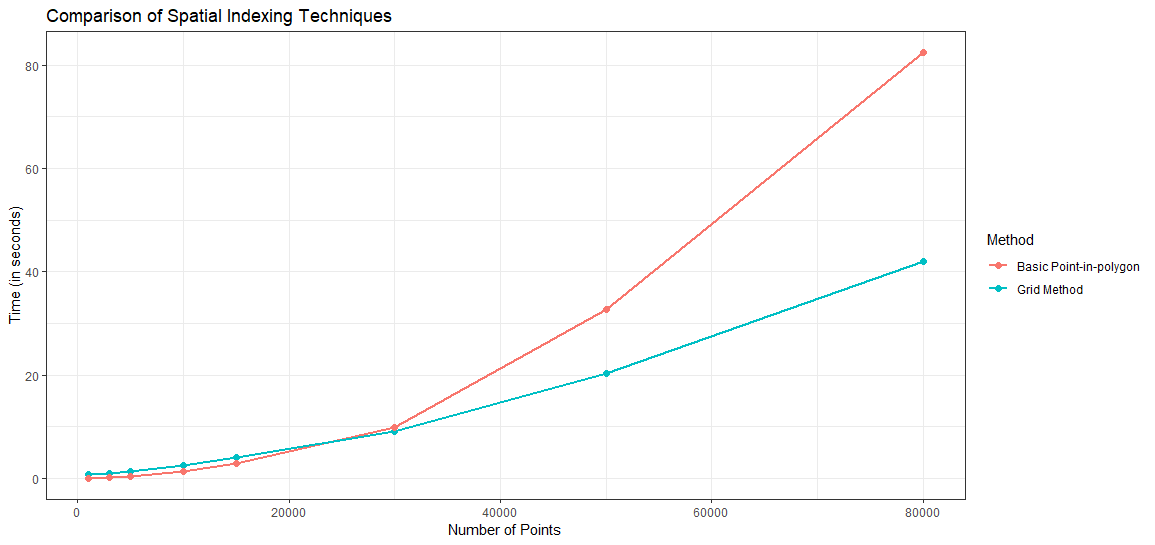
\includegraphics[width=1\linewidth]{Sections/tables and figures/Example Spatial Indexing Techniques} \caption{Spatial Index Time Comparison}\label{fig:Spatial Indexing Process}
\end{figure}

\begin{figure}[h]
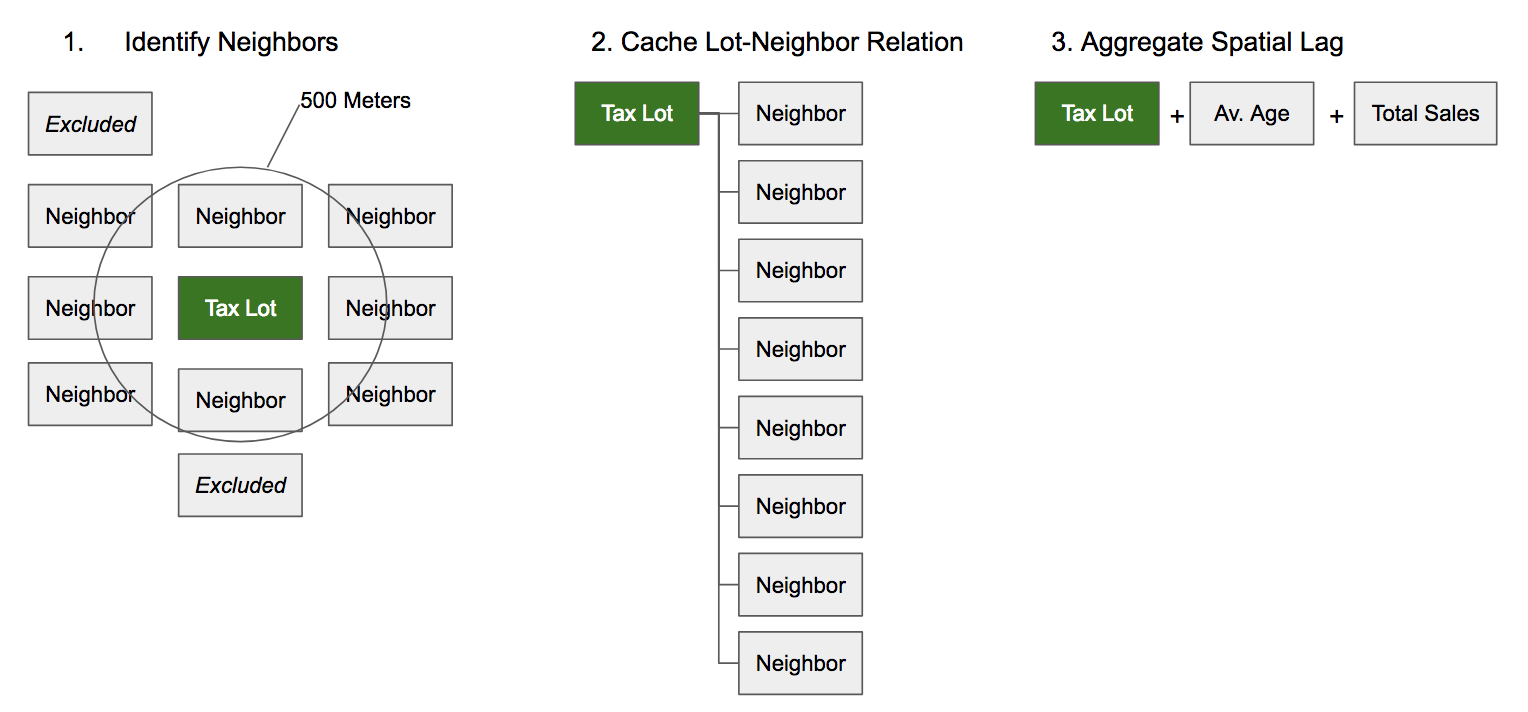
\includegraphics[width=1\linewidth]{Sections/tables and figures/Spatial Lag Creation} \caption{Spatial Lag Feature Creation Process}\label{fig:Spatial Lag Feataure Process}
\end{figure}

Next, we used the spatial index to create spatial lag features. One
advantage of using spatial lags is the rich number of potential features
which can be engineered. Spatial lags can be weighted based on a
distance function, e.g., physically closer observations can be given
more weight. For our modeling purposes, we created two sets of features:
distance weighted features (denoted with a "\_dist" in Appendix A Table
\ref{tab:AppendixA}) and simple average features (denoted with "\_basic"
in Appendix A Table \ref{tab:AppendixA}). SMA and EMA as well as percent
changes were also calculated. Temporal and spatial derivatives of the
Spatial Lag features presented in Table \ref{tab:summarySLfeats} were
also added to the model, including: variables weighted by euclidean
distance (``dist''), basic averages of the spatial lag radius (``basic
mean''), Simple Moving Averages (``SMA'') for 2 years, 3 years and 5
years, exponential moving averages (``EMA'') for 2 years, 3 years and 5
years, and year-over-year percent changes for all variables (``perc
change''). In total, the spatial lag feature engineering process input
92 variables and output 194 variables. A summary of the Spatial Lag
features are presented in Appendix A Table \ref{tab:AppendixA}.

\begin{table}

\caption{\label{tab:Table 3}\label{tab:summarySLfeats} Summary of Spatial Lag Features (See Appendix A for full list)}
\centering
\resizebox{\linewidth}{!}{
\begin{tabular}[t]{l}
\toprule
Spatial Lag Features\\
\midrule
Radius Total Sold In Year\\
Radius Average Years Since Last Sale\\
Radius Res Units Sold In Year\\
Radius All Units Sold In Year\\
Radius SF Sold In Year\\
\addlinespace
Radius Total Sold In Year sum over 2 years\\
Radius Average Years Since Last Sale sum over 2 years\\
Radius Res Units Sold In Year sum over 2 years\\
Radius All Units Sold In Year sum over 2 years\\
Radius SF Sold In Year sum over 2 years\\
\addlinespace
Radius Total Sold In Year percent change\\
Radius Average Years Since Last Sale percent change\\
Radius Res Units Sold In Year percent change\\
Radius All Units Sold In Year percent change\\
Radius SF Sold In Year percent change\\
\addlinespace
Radius Total Sold In Year sum over 2 years percent change\\
Radius Average Years Since Last Sale sum over 2 years percent change\\
Radius Res Units Sold In Year sum over 2 years percent change\\
Radius All Units Sold In Year sum over 2 years percent change\\
Radius SF Sold In Year sum over 2 years percent change\\
\bottomrule
\end{tabular}}
\end{table}

\hypertarget{outcome-variables}{%
\subsection{Outcome Variables}\label{outcome-variables}}

The final step in creating the modeling data is to define the outcome
variables. For our purposes, we create two dependent variables:

\begin{enumerate}
\def\labelenumi{\arabic{enumi})}
\tightlist
\item
  \textbf{Sold.} whether a tax lot sold in a given year. Used in the
  Probability of Sale classification model.
\item
  \textbf{Sale Price.} The price-per-square foot associated with a
  transaction, if a sale took place. Used in the Sale Price Regression
  model.
\end{enumerate}

\noindent Table \ref{tab:OutcomeDistro} describes the distributions of
both outcome variables:

\begin{table}

\caption{\label{tab:table 4}\label{tab:OutcomeDistro} Distributions for Outcome Variables}
\centering
\begin{tabular}[t]{lll}
\toprule
  & Sold & Sale Price per SF\\
\midrule
Min. & 0.00 & 0.0\\
1st Qu. & 0.00 & 163.5\\
Median & 0.00 & 375.2\\
Mean & 0.04 & 644.8\\
3rd Qu. & 0.00 & 783.3\\
Max. & 1.00 & 83,598.7\\
\bottomrule
\end{tabular}
\end{table}

\hypertarget{algorithm}{%
\subsection{Algorithm}\label{algorithm}}

Previous works (see: Antipov and Pokryshevskaya (2012); also
Schernthanner H. (2016)) have found the Random Forest algorithm (Breiman
2001) suitable to prediction tasks involving real estate. While
algorithms exist that may marginally outperform Random Forest in terms
of predictive accuracy (such as neural networks and functional gradient
descent algorithms), Random Forest is highly scalable and
parallelizable, and therefore a natural choice for comparing different
feature engineering strategies. For these reasons and more outlined
below, we select Random Forrest as the primary algorithm for comparrison
in this paper.

Random Forest can be used for both classification and regression tasks,
both of which we undertake in this paper. The Random Forest algorithm
works by generating a large number of independent classification or
regression decision trees and then employing majority voting (for
classification) or averaging (for regression) to generate predictions.
Over a data set of N rows by M predictors, a bootstrap sample of the
data is chosen (n \textless{} N) as well as a subset of the predictors
(m \textless{} M). Individual decision/regression trees are built on the
n by m sample. Because the trees can be built independently (and not
sequentially, as is the case with most functional gradient descent
algorithms), the tree building process can be executed in parallel
across an arbitrary number of computer cores. With a sufficiently large
number of cores, the model training time can be significantly reduced.
This provides a highly accurate, robust prediction model that avoids
many of the drawbacks of traditional parametric techniques, such as OLS.

The primary advantages to using Random Forest with real estate data are:

\begin{enumerate}
\def\labelenumi{\arabic{enumi}.}
\tightlist
\item
  Can handle an arbitrarily large number of variables while avoiding the
  curse of dimensionality associated with regression techniques.
  Increasing the number of predictors in a multiple regression can
  quickly lead to over-fitting.
\item
  Can accommodate categorical variables with many levels. Real estate
  data often contains information describing the location of the
  property, or the property itself, as one of a large set of possible
  choices, such as neighborhood, county, census tract, district,
  property type, and zoning information. Because factors need to be
  recoded as individual dummy variables in the model building process,
  factors with many levels will quickly encounter the curse of
  dimensionality in multiple regression techniques.
\item
  Appropriately handles missing data. Predictions can be made with the
  parts of the tree which are successfully built, and therefore, there
  is no need to filter out incomplete observations or impute missing
  values. Since much real estate data is self reported, incomplete
  fields are common in the data.
\item
  Robust against outliers. Because of bootstrap sampling, outliers
  appear in individual trees less often, and therefore, are reduced in
  terms of importance. Real estate data, especially with regards to
  pricing, tends to contain outliers. For example, the dependent
  variable in one of our models, Sale Price (see: Table 7), shows a
  clear divergence in median and mean, as well as a maximum
  significantly higher than the third quartile.
\item
  Can recognize non-linear relationships in data, which is useful when
  modeling spatial relationships.
\item
  Is not affected by co-linearity in the data. This is highly valuable
  as real estate data can be highly correlated.
\item
  The algorithm can be parallelized and is relatively fast compared to
  neural networks and functional gradient descent algorithms.
\end{enumerate}

To run the model, we have chosen the h2o.randomForest function from the
h2o R open source library. The h2o implementation of the Random Forest
algorithm is particularly well-suited for high parallelization. For more
information, see: \url{https://www.h2o.ai/}.

\hypertarget{model-validation}{%
\subsection{Model Validation}\label{model-validation}}

The goal of the predictive models are to be able to successfully predict
both the probability and amount of real estate sales into the near
future. As such, our models will use out-of-time validation to assess
performance. As shown in Figure \ref{fig:Train Test Validate} The models
will be trained using data from 2003-2015. 2016 modeling data will be
used during the model training process as cross-validation data.
Finally, we will score our model using 2017 as a held-out sample. Using
out-of-time validation should ensure that the models generalize well
into the immediate future.

\begin{figure}[h]
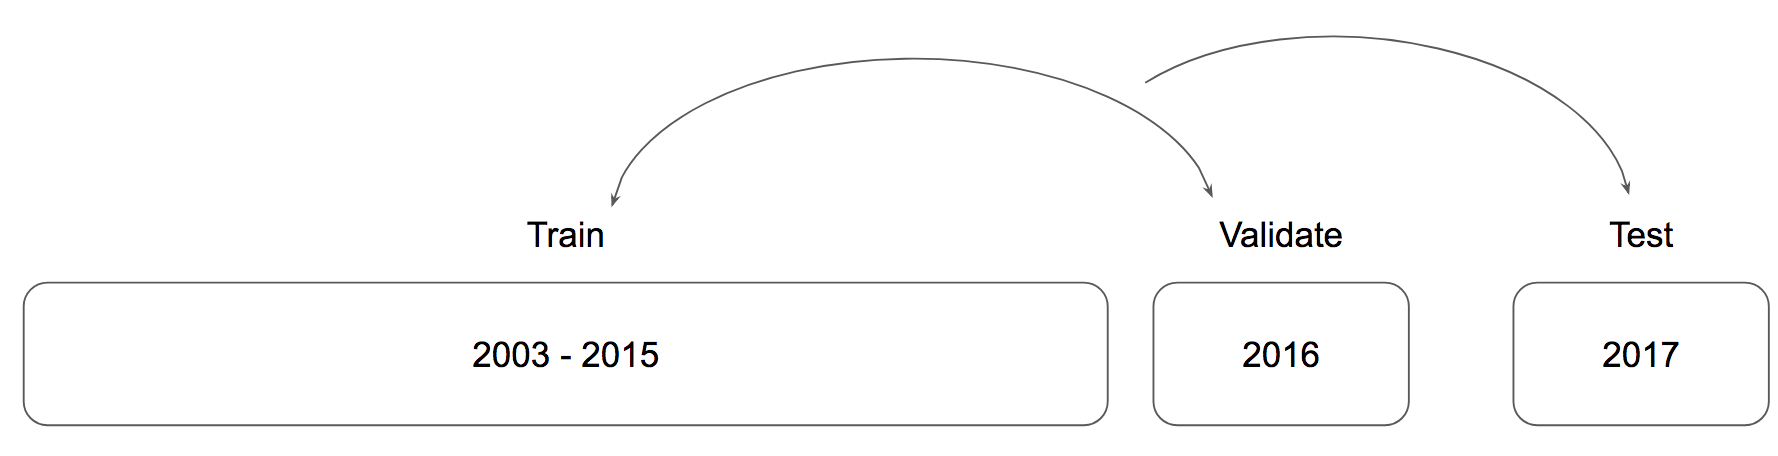
\includegraphics[width=1\linewidth]{Sections/tables and figures/Train Validate Test} \caption{Out-of-time validation}\label{fig:Train Test Validate}
\end{figure}

\hypertarget{variable-selection}{%
\subsection{Variable Selection}\label{variable-selection}}

For ease of processing and to improve the ability of the model to
generalize into the future, a variable selection step is added to the
modeling process. A Random Forest model is first trained on a 1\%
sub-sample of the modeling data. Variable importance of the resulting
model is calculated using the technique proposed by Friedman (2001),
i.e., for a collection of decision trees \([T_m]_{1}^{m}\):

\[
  \hat{I_{j}^{2}} = \frac{1}{M} \sum_{m=1}^{M}\hat{I_{j}^{2}}(T_m)
\]

Where influence \(I\) for variable \(j\) is calculated as the sum of
corresponding improvements in squared-error for node tree \(T\). After
calculating variable importance for the model data subset, the variables
are rank-ordered by descending importance. Variables which account for
80\% of the total variable importance are chosen to advance to the model
training round on the full modeling data sets.

\hypertarget{evaluation-metrics}{%
\subsection{Evaluation Metrics}\label{evaluation-metrics}}

We have chosen evaluation metrics that will allow us to easily compare
the performance of the models against other models with the same outcome
variable. The classification models (Probability of Sale) will be
compared using Area Under the ROC Curve (AUC). The regression models
(Sale Price) will be compared using Root Mean Squared Error (RMSE). Both
evaluation metrics are common for their respective outcome variable
types, and as such will be useful for comparing within model-groups.

\hypertarget{area-under-roc-curve-auc}{%
\subsubsection{Area Under ROC Curve
(AUC)}\label{area-under-roc-curve-auc}}

A classification model typically outputs a probability that a given row
in the data belongs to a group. In the case of binary classification,
the value falls between 0 and 1. There are many techniques for
determining the cut off threshold for classification; a typical method
is to assign anything above a 0.5 into the ``1'' or positive class. An
ROC curve (receiver operating characteristic curve) plots the True
Positive Rate vs.~the False Positive rate at different classification
thresholds; it is a measurement of the performance of a classification
model across all possible thresholds, and therefore sidesteps the need
to arbitrarily assign a cutoff.

Area Under the ROC Curve, or AUC measures the entire two-dimensional
area underneath the ROC curve. It is the integration of the curve from
(0,0) to (1,1), defined as \(AUC = \int_{(0,0)}^{(1,1)} f(x)dx\).

AUC provides a relatively standard measure of performance across all
possible classification thresholds, and can be interpreted as the
probability that the model ranks a random positive example more highly
than a random negative example. A value of 0.5 represents a perfectly
random model, while a value of 1.0 represents a model that can perfectly
discriminate between the two classes. AUC is useful for comparing
classification models against one another because they are both scale
and threshold-invariant.

One of the drawbacks to AUC is that is does not describe the trade-offs
between false positives and false negatives. In certain circumstances, a
false positive might be considerably less desirable than a false
negative, or vice-versa. For our purposes, we rank false positives and
false negatives as equally undesirable outcomes.

\hypertarget{root-mean-squared-error}{%
\subsubsection{Root Mean Squared Error}\label{root-mean-squared-error}}

The Root Mean Squared Error (RMSE) is a common measurement of the
differences between values predicted by a regression model and the
observed values. It is formally defined as
\(RMSE = \sqrt{ \frac{\sum_{1}^{T} (\hat{y}_t - y_t)^2}{T} }\), where
\(\hat{y}\) represents the prediction and \(y\) represents the observed
value at observation \(t\).

Lower RMSE scores are typically more desirable. An RMSE value of 0 would
indicate a perfect fit to the data. RMSE can be difficult to interpret
on its own, however, it is useful for comparing models with similar
outcome variables. In our case, the outcome variables (Sales Price per
Square Foot) are consistent across modeling data sets, and therefore can
be reasonably compared using RMSE.

\hypertarget{results}{%
\section{Results}\label{results}}

\hypertarget{sale-price-model}{%
\subsection{Sale Price Model}\label{sale-price-model}}

The Root Mean Squared Error (RMSE) of all models predicting Sale Price
is analyzed at the data set, Borough and Building Type level. Table
\ref{tab:SalePriceEval} shows the average ranking by model type as well
as the distribution of models that ranked first, second and third for
each respective Borough/Building Type combination using RMSE as a
ranking metric. If we rank the models by performance for each Borough,
Building Type combination, we find that the Spatial Lag models
outperform the Zip Code models in 72\% of cases with an average
model-rank of 2.11 and 2.5, respectively. The Base modeling data set
tends to outperform both enriched datasets, suggesting an issue with
model over-fit in some areas. Despite this, the Spatial Lag feature data
sets outperform all other models for certain building types, notably for
Type A buildings (One Family Dwellings) and Type L buildings (Lofts) in
Manhattan as well as Type O Buildings (Office) in Queens as shown in
\ref{fig:RMSE by boro and build type}.

\begin{table}

\caption{\label{tab:Sale Price Evaluations}\label{tab:SalePriceEval} Sale Price Model RMSE For Validation and Test Hold-out Data}
\centering
\begin{tabular}[t]{lrrr}
\toprule
type & base & zip & spatial lag\\
\midrule
Validation & 280.6314 & 297.9717 & 286.2295\\
Test & 287.8305 & 300.6031 & 297.9202\\
\bottomrule
\end{tabular}
\end{table}

Figure \ref{fig:RMSE by boro and build type} shows RMSE by Model,
faceted by Borough across the y-axis and Building Type across the x-axis
(See Table 2 for a description of building type codes). We make the
following observations from Figure
\ref{fig:RMSE by boro and build type}:

\begin{itemize}
\tightlist
\item
  The Spatial Lag modeling data outperforms both Base and Zip Code in 6
  cases, notably for Type A buildings (One Family Dwellings) and Type L
  buildings (Lofts) in Manhattan as well as Type O Buildings (Office) in
  Queens
\item
  It is generally harder to predict sale prices in Manhattan compared to
  other Boroughs
\item
  The ``residential'' building Types A (One Family Dwellings), B (Two
  Family Dwellings), C (Walk Up Apartments) and D (Elevator Apartments)
  have generally lower RMSE scores compared to the non-residential types
\end{itemize}

\begin{figure}[h]
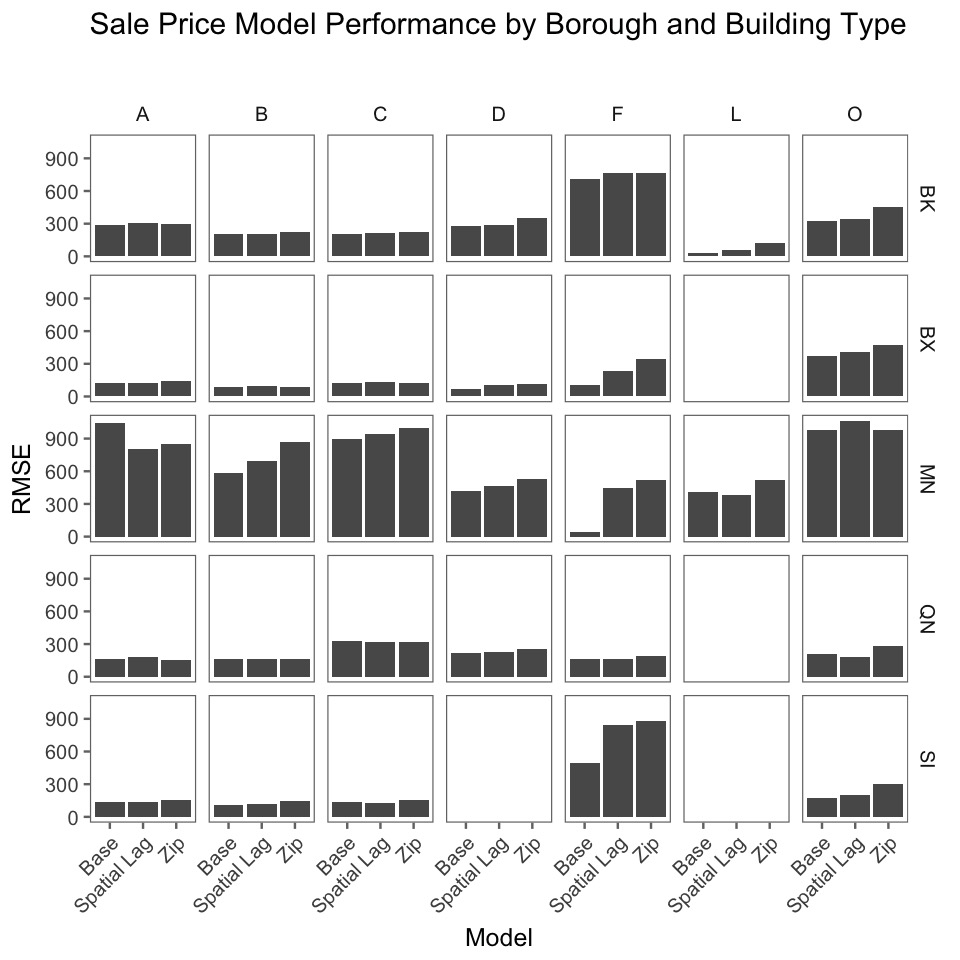
\includegraphics[width=1\linewidth]{Sections/tables and figures/RMSE by boro and build type} \caption{RMSE By Borough and Building Type}\label{fig:RMSE by boro and build type}
\end{figure}

\begin{table}

\caption{\label{tab:Sale Price Model Rank Distributions}\label{tab:SalePriceModelRank} Sale Price Model Rankings, RMSE by Borough and Building Type}
\centering
\begin{tabular}[t]{llllr}
\toprule
Model Rank & 1 & 2 & 3 & Average Rank\\
\midrule
Base & 22.2\% & 9.3\% & 1.9\% & 1.39\\
Spatial Lag & 5.6\% & 18.5\% & 9.3\% & 2.11\\
Zip & 5.6\% & 5.6\% & 22.2\% & 2.50\\
\bottomrule
\end{tabular}
\end{table}

\hypertarget{probability-of-sale-model}{%
\subsection{Probability of Sale Model}\label{probability-of-sale-model}}

Similar to the results found in the Sale Price models, using Area Under
the ROC Curve (AUC) as an evaluation metric, we find the Spatial Lag
model performs better on the hold-out validation data compared to the
Zip Code modeling data, as shown in Table \ref{tab:ProbSaleModelAUC}.
The Base Modeling data continues to outperform the Spatial Lag and Zip
Code modeling data overall, however, when broken down by Borough and
Building Type, some interesting patterns emerge.

\begin{table}

\caption{\label{tab:Prob Model AUC}\label{tab:ProbSaleModelAUC} Probability of Sale Model AUC}
\centering
\begin{tabular}[t]{lrrr}
\toprule
Model AUC & Base & Zip & Spatial Lag\\
\midrule
Validation & 0.832 & 0.8292 & 0.8287\\
Test & 0.830 & 0.8246 & 0.8279\\
\bottomrule
\end{tabular}
\end{table}

Looking at the predictions by the models made on the 2017 validation
hold-out data, we see the Spatial Lag model performs best of any model
for three out of five Boroughs: Manhattan, Bronx and Staten Island (see:
Table \ref{tab:ProbSaleModelAUCbyBoro}).

\begin{table}

\caption{\label{tab:Prob Model AUC by Boro}\label{tab:ProbSaleModelAUCbyBoro} Probability of Sale Models AUC by Borough}
\centering
\begin{tabular}[t]{lrrrrr}
\toprule
Model & BK & BX & MN & QN & SI\\
\midrule
Base & 0.8309 & 0.8288 & 0.7926 & 0.8338 & 0.8336\\
Zip & 0.8234 & 0.8215 & 0.7796 & 0.8283 & 0.8281\\
Spatial Lag & 0.8257 & 0.8312 & 0.8031 & 0.8327 & 0.8348\\
\bottomrule
\end{tabular}
\end{table}

Figure \ref{fig:AUC by boro and build type} shows a breakdown of model
AUC faceted along the x-axis by Building Type and along the y-axis by
Borough. The coloring indicated by how much a model's AUC diverges from
the cell average.

\begin{figure}[h]
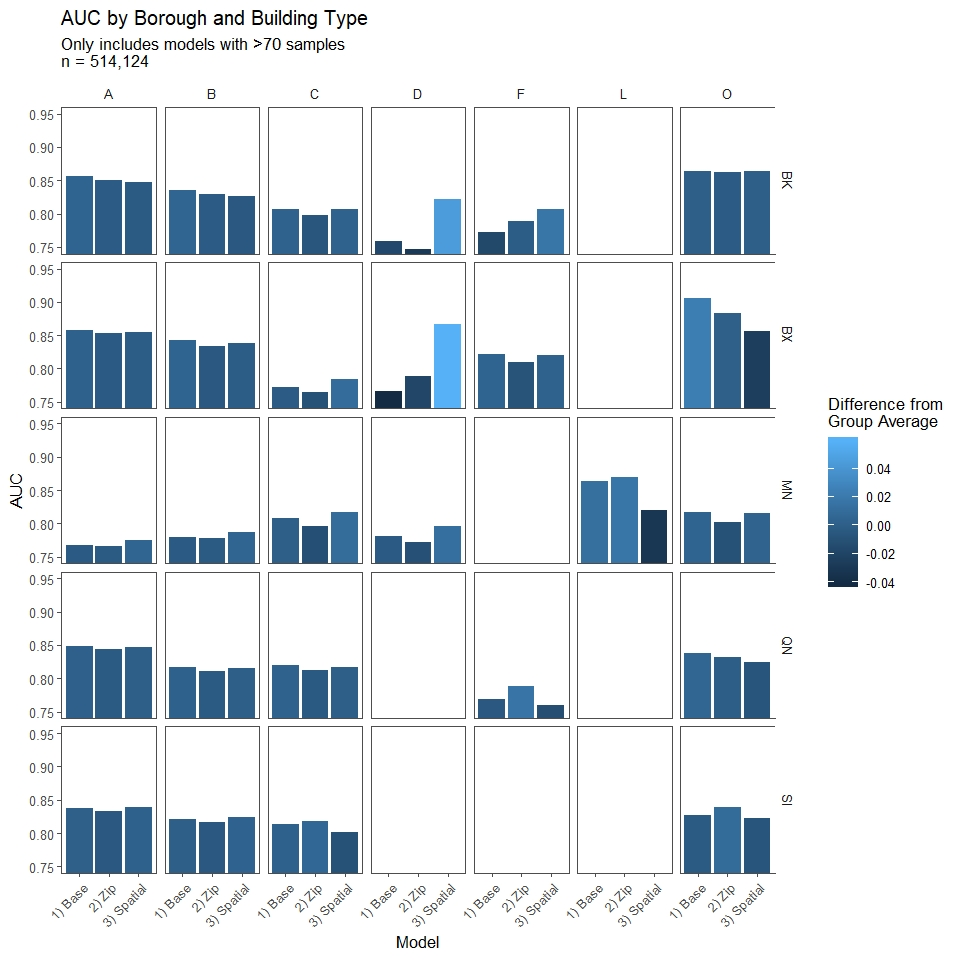
\includegraphics[width=1\linewidth]{Sections/tables and figures/AUC by boro and build type} \caption{AUC By Borough and Building Type}\label{fig:AUC by boro and build type}
\end{figure}

We make the following observations about Figure
\ref{fig:AUC by boro and build type}:

\begin{itemize}
\tightlist
\item
  The Spatial Lag model outperforms all other models for Elevator
  Buildings (Type D), particularly in the Bronx
\item
  The Probability of Sale model tends to perform poorly in Manhattan
  vs.~other Boroughs
\item
  However, the Spatial Lag model performs well in Manhattan for the
  residential building types (A, B, C and D)
\end{itemize}

If we rank model the probability models' performance for each Borough
and Building Type, we see that the Spatial Lag models consistently
outperform the Zip Code models, as shown in Table
\ref{tab:ProbModelAUCRank}

\begin{table}

\caption{\label{tab:Prob Model AUC Average Rank}\label{tab:ProbModelAUCRank} Distribution and Average Model Rank for Probability of Sale by AUC across Borough and Building Types}
\centering
\begin{tabular}[t]{llllr}
\toprule
Model Rank & 1 & 2 & 3 & Average Rank\\
\midrule
Base & 16.2\% & 12.0\% & 5.1\% & 2.22\\
Spatial Lag & 11.1\% & 13.7\% & 8.5\% & 2.09\\
Zip & 6.0\% & 7.7\% & 19.7\% & 1.69\\
\bottomrule
\end{tabular}
\end{table}

\hypertarget{future-research-and-conclusions}{%
\section{Future Research and
Conclusions}\label{future-research-and-conclusions}}

\hypertarget{future-research}{%
\subsection{Future Research}\label{future-research}}

This research has shown that spatial-lag features can be worthwhile
additions to machine learning predictive models in certain
circumstances. There are several areas that could be further explored
regarding spatial lag features, some of which are mentioned below.

First, it became apparent in the research that generalization was a
problem for the models overall, likely due to overfitting of the
training data. Further research into proper varibale selection could be
one remedy for such issues.

Additionally, the spatial lag features seemd to perform best for outer
boroughs (non-Manhattan) and for smaller, residential building types.
One possible explanation for this is that these types of assetts are
considerably more numerous and homogenous. It is possible that a 500
meter radius, which was arbitrarily chosen, works best for this type of
asset. Fotheringham (2015) used an ``Adaptive Bandwidth'' technique to
adjust the spatial lag radius based on cross-validation. research into
applying a similar technique to this research could be valuable.

Finally, this research aimed to predict real estate transactions 1 year
into the future. While this is a promising start, 1-year of lead time
may not be sufficient to respond to growing gentirifaction challenges.
In addition, modeling at the annual level could be improved to quartlery
or monthly, given that the sales data contains date information down to
the day. To make this system practial for combatting displacement, it
may be helpful to predict at a more granular level and further into the
future.

\hypertarget{conclusion}{%
\subsection{Conclusion}\label{conclusion}}

Gentification is largely beneficial to societies and communities,
however, the downside should not be overlooked. Displacement causes
Economic Exclusion, which over time can contribute to rising Income
Inequality. Combatting displacement allows communities to benefit from
gentrification without suffering the negative consequences. One way to
practically combat displacement is to predict gentirification, which
this paper has attempted to do.

Spatial lags, typically seen in geographically weighted regression, were
employed successfully to enhance the predictive power of machine
learning models. The features suffered in some areas do to modeling and
data shortcomings, but overall we found that spatial lags outperform
zip-code level aggregations, and perform quite well for specific asset
types and geographic locations, particularly residential buildings
outside of Manhattan.

While this research is not intended to serve as a full early-warining
system for gentrification and displacmenet, it is a step in that
direction. More research is needed to help address the challenges faced
by city planners and governments trying to help incumbent residents reap
the benefits of local investments. Income inequallity is a complicated
and grave issue of our time, but new tools and tecnhiques to inform and
prevent give a hope for a more equitable future.

\newpage

\hypertarget{appendix-a-full-list-of-spatial-lag-features}{%
\section{Appendix A: Full List of Spatial Lag
Features}\label{appendix-a-full-list-of-spatial-lag-features}}

\begin{table}

\caption{\label{tab:Appendix A}\label{tab:AppendixA} Appendix A: All Spatial Lag Features}
\centering
\resizebox{\linewidth}{!}{
\begin{tabular}[t]{lllll}
\toprule
Feature & Min & Median & Mean & Max\\
\midrule
Radius\_Total\_Sold\_In\_Year & 1.00 & 20.00 & 24.00 & 201.00\\
Radius\_Average\_Years\_Since\_Last\_Sale & 1.00 & 4.43 & 4.27 & 14.00\\
Radius\_Res\_Units\_Sold\_In\_Year & 0.00 & 226.00 & 289.10 & 2,920.00\\
Radius\_All\_Units\_Sold\_In\_Year & 0.00 & 255.00 & 325.94 & 2,923.00\\
Radius\_SF\_Sold\_In\_Year & 0.00 & 259,403.00 & 430,891.57 & 8,603,639.00\\
\addlinespace
Radius\_Total\_Sold\_In\_Year\_sum\_over\_2\_years & 2.00 & 41.00 & 48.15 & 256.00\\
Radius\_Average\_Years\_Since\_Last\_Sale\_sum\_over\_2\_years & 2.00 & 9.25 & 8.70 & 26.00\\
Radius\_Res\_Units\_Sold\_In\_Year\_sum\_over\_2\_years & 0.00 & 493.00 & 584.67 & 3,397.00\\
Radius\_All\_Units\_Sold\_In\_Year\_sum\_over\_2\_years & 1.00 & 555.00 & 660.67 & 4,265.00\\
Radius\_SF\_Sold\_In\_Year\_sum\_over\_2\_years & 2,917.00 & 580,947.00 & 872,816.44 & 14,036,469.00\\
\addlinespace
Radius\_Total\_Sold\_In\_Year\_percent\_change & -0.99 & 0.00 & 0.27 & 77.00\\
Radius\_Average\_Years\_Since\_Last\_Sale\_percent\_change & -0.91 & 0.13 & 0.26 & 8.00\\
Radius\_Res\_Units\_Sold\_In\_Year\_percent\_change & -1.00 & -0.04 & Inf & Inf\\
Radius\_All\_Units\_Sold\_In\_Year\_percent\_change & -1.00 & -0.04 & Inf & Inf\\
Radius\_SF\_Sold\_In\_Year\_percent\_change & -1.00 & -0.02 & Inf & Inf\\
\addlinespace
Radius\_Total\_Sold\_In\_Year\_sum\_over\_2\_years\_percent\_change & -0.96 & -0.03 & 0.03 & 15.00\\
Radius\_Average\_Years\_Since\_Last\_Sale\_sum\_over\_2\_years\_percent\_change & -0.72 & 0.12 & 0.17 & 2.50\\
Radius\_Res\_Units\_Sold\_In\_Year\_sum\_over\_2\_years\_percent\_change & -1.00 & -0.04 & Inf & Inf\\
Radius\_All\_Units\_Sold\_In\_Year\_sum\_over\_2\_years\_percent\_change & -0.99 & -0.04 & 0.12 & 84.00\\
Radius\_SF\_Sold\_In\_Year\_sum\_over\_2\_years\_percent\_change & -0.98 & -0.04 & 0.18 & 361.55\\
\addlinespace
Percent\_Com\_dist & 0.00 & 0.04 & 0.07 & 0.56\\
Percent\_Res\_dist & 0.00 & 0.46 & 0.43 & 0.66\\
Percent\_Office\_dist & 0.00 & 0.01 & 0.03 & 0.48\\
Percent\_Retail\_dist & 0.00 & 0.02 & 0.02 & 0.09\\
Percent\_Garage\_dist & 0.00 & 0.00 & 0.00 & 0.27\\
\addlinespace
Percent\_Storage\_dist & 0.00 & 0.00 & 0.01 & 0.26\\
Percent\_Factory\_dist & 0.00 & 0.00 & 0.00 & 0.04\\
Percent\_Other\_dist & 0.00 & 0.00 & 0.00 & 0.09\\
Percent\_Com\_basic\_mean & 0.00 & 0.04 & 0.07 & 0.54\\
Percent\_Res\_basic\_mean & 0.00 & 0.46 & 0.43 & 0.66\\
\addlinespace
Percent\_Office\_basic\_mean & 0.00 & 0.01 & 0.03 & 0.44\\
Percent\_Retail\_basic\_mean & 0.00 & 0.02 & 0.02 & 0.08\\
Percent\_Garage\_basic\_mean & 0.00 & 0.00 & 0.00 & 0.29\\
Percent\_Storage\_basic\_mean & 0.00 & 0.00 & 0.01 & 0.23\\
Percent\_Factory\_basic\_mean & 0.00 & 0.00 & 0.00 & 0.03\\
\addlinespace
Percent\_Other\_basic\_mean & 0.00 & 0.00 & 0.00 & 0.04\\
Percent\_Com\_dist\_perc\_change & -0.90 & 0.00 & 0.00 & 6.18\\
Percent\_Res\_dist\_perc\_change & -0.50 & 0.00 & 0.03 & 36.73\\
Percent\_Office\_dist\_perc\_change & -1.00 & 0.00 & Inf & Inf\\
Percent\_Retail\_dist\_perc\_change & -0.82 & 0.00 & Inf & Inf\\
\addlinespace
Percent\_Garage\_dist\_perc\_change & -1.00 & 0.00 & Inf & Inf\\
Percent\_Storage\_dist\_perc\_change & -1.00 & -0.01 & Inf & Inf\\
Percent\_Factory\_dist\_perc\_change & -1.00 & 0.00 & Inf & Inf\\
Percent\_Other\_dist\_perc\_change & -1.00 & 0.00 & Inf & Inf\\
SMA\_Price\_2\_year\_dist & 0.00 & 400.01 & 496.30 & 3,816.57\\
\addlinespace
SMA\_Price\_3\_year\_dist & 0.00 & 396.94 & 492.00 & 3,816.57\\
SMA\_Price\_5\_year\_dist & 8.83 & 425.55 & 515.29 & 3,877.53\\
Percent\_Change\_SMA\_2\_dist & -0.13 & 0.03 & 552.33 & 804,350.67\\
Percent\_Change\_SMA\_5\_dist & -0.09 & 0.02 & 317.46 & 322,504.58\\
EMA\_Price\_2\_year\_dist & 0.00 & 378.63 & 475.54 & 3,431.17\\
\addlinespace
EMA\_Price\_3\_year\_dist & 8.83 & 382.25 & 476.05 & 3,296.46\\
EMA\_Price\_5\_year\_dist & 7.88 & 386.34 & 468.91 & 2,813.34\\
Percent\_Change\_EMA\_2\_dist & -0.09 & 0.06 & 346.51 & 480,829.57\\
Percent\_Change\_EMA\_5\_dist & -0.02 & 0.06 & 303.55 & 273,458.42\\
SMA\_Price\_2\_year\_basic\_mean & 0.02 & 412.46 & 496.75 & 2,509.79\\
\addlinespace
SMA\_Price\_3\_year\_basic\_mean & 0.02 & 409.00 & 492.43 & 2,509.79\\
SMA\_Price\_5\_year\_basic\_mean & 17.16 & 443.34 & 515.67 & 2,621.01\\
Percent\_Change\_SMA\_2\_basic\_mean & -0.13 & 0.04 & 543.51 & 393,749.99\\
Percent\_Change\_SMA\_5\_basic\_mean & -0.09 & 0.03 & 312.46 & 157,500.00\\
EMA\_Price\_2\_year\_basic\_mean & 0.02 & 390.30 & 475.96 & 2,259.21\\
\addlinespace
EMA\_Price\_3\_year\_basic\_mean & 11.39 & 393.25 & 476.45 & 2,136.36\\
EMA\_Price\_5\_year\_basic\_mean & 15.30 & 402.06 & 469.09 & 1,848.27\\
Percent\_Change\_EMA\_2\_basic\_mean & -0.09 & 0.06 & 340.89 & 235,378.24\\
Percent\_Change\_EMA\_5\_basic\_mean & -0.02 & 0.06 & 296.78 & 133,547.59\\
SMA\_Price\_2\_year\_dist\_perc\_change & -0.74 & 0.05 & 0.17 & 10,540.56\\
\addlinespace
SMA\_Price\_3\_year\_dist\_perc\_change & -0.74 & 0.05 & 0.17 & 10,540.56\\
SMA\_Price\_5\_year\_dist\_perc\_change & -0.74 & 0.04 & 0.06 & 15.37\\
Percent\_Change\_SMA\_2\_dist\_perc\_change & -Inf & -0.24 & NaN & Inf\\
Percent\_Change\_SMA\_5\_dist\_perc\_change & -Inf & -0.14 & NaN & Inf\\
EMA\_Price\_2\_year\_dist\_perc\_change & -0.74 & 0.06 & 0.18 & 10,540.57\\
\addlinespace
EMA\_Price\_3\_year\_dist\_perc\_change & -0.73 & 0.06 & 0.08 & 15.06\\
EMA\_Price\_5\_year\_dist\_perc\_change & -0.63 & 0.06 & 0.07 & 12.04\\
Percent\_Change\_EMA\_2\_dist\_perc\_change & -Inf & -0.13 & NaN & Inf\\
Percent\_Change\_EMA\_5\_dist\_perc\_change & -556.60 & -0.10 & Inf & Inf\\
SMA\_Price\_2\_year\_basic\_mean\_perc\_change & -0.55 & 0.05 & 0.12 & 9,375.77\\
\addlinespace
SMA\_Price\_3\_year\_basic\_mean\_perc\_change & -0.55 & 0.05 & 0.11 & 9,375.77\\
SMA\_Price\_5\_year\_basic\_mean\_perc\_change & -0.50 & 0.04 & 0.06 & 5.90\\
Percent\_Change\_SMA\_2\_basic\_mean\_perc\_change & -Inf & -0.19 & NaN & Inf\\
Percent\_Change\_SMA\_5\_basic\_mean\_perc\_change & -Inf & -0.12 & NaN & Inf\\
EMA\_Price\_2\_year\_basic\_mean\_perc\_change & -0.53 & 0.06 & 0.12 & 9,375.78\\
\addlinespace
EMA\_Price\_3\_year\_basic\_mean\_perc\_change & -0.47 & 0.06 & 0.08 & 23.54\\
EMA\_Price\_5\_year\_basic\_mean\_perc\_change & -0.37 & 0.06 & 0.07 & 4.81\\
Percent\_Change\_EMA\_2\_basic\_mean\_perc\_change & -Inf & -0.13 & NaN & Inf\\
Percent\_Change\_EMA\_5\_basic\_mean\_perc\_change & -136.59 & -0.11 & Inf & Inf\\
\bottomrule
\end{tabular}}
\end{table}

\hypertarget{references}{%
\section*{References}\label{references}}
\addcontentsline{toc}{section}{References}

\hypertarget{refs}{}
\leavevmode\hypertarget{ref-Almanie2015}{}%
Almanie, R.; Lor, T.; Mirza. 2015. ``Crime Prediction Based on Crime
Types and Using Spatial and Temporal Criminal Hotspots.''
\emph{International Journal of Data Mining \& Knowledge Management
Process (IJDKP)} 5 (4).

\leavevmode\hypertarget{ref-antipov12}{}%
Antipov, Evgeny A., and Elena B. Pokryshevskaya. 2012. ``Mass Appraisal
of Residential Apartments: An Application of Random Forest for Valuation
and a Cart-Based Approach for Model Diagnostics.'' \emph{Expert Systems
with Applications}.

\leavevmode\hypertarget{ref-Pollack2010}{}%
Barry Bluestone \& Chase Billingham, Stephanie Pollack \&. 2010.
``Maintaining Diversity in America's Transit-Rich Neighborhoods: Tools
for Equitable Neighborhood Change.'' \emph{New England Community
Developments, Federal Reserve Bank of Boston}, 1--6.

\leavevmode\hypertarget{ref-Batty2013}{}%
Batty, Michael. 2013. ``The New Science of Cities.'' \emph{MIT Press}.

\leavevmode\hypertarget{ref-Breiman2001}{}%
Breiman, L. 2001. ``Random Forests.'' \emph{Machine Learning} 45 (1):
5--32.

\leavevmode\hypertarget{ref-Chapple2009}{}%
Chapple, Karen. 2009. ``Mapping Susceptibility to Gentrification: The
Early Warning Toolkit.'' \emph{Berkeley, CA: Center for Community
Innovation.}

\leavevmode\hypertarget{ref-Chapple2016}{}%
Chapple, Miriam, Karen; Zuk. 2016. ``Forewarned: The Use of Neighborhood
Early Warning Systems for Gentrification and Displacement.''
\emph{Cityscape: A Journal of Policy Development and Research} 18 (3).

\leavevmode\hypertarget{ref-Clay1979}{}%
Clay, Phillip L. 1979. \emph{Neighborhood Renewal: Middle-Class
Resettlement and Incumbent Upgrading in American Neighborhoods}.
Lexington Books.

\leavevmode\hypertarget{ref-Springer2017}{}%
d'Amato, Tom, Maurizio; Kauko, ed. 2017. \emph{Advances in Automated
Valuation Modeling}. Springer International Publishing.

\leavevmode\hypertarget{ref-Dietzell2014}{}%
Dietzell, Nicole; Schäfers, Marian Alexander; Braun. 2014.
``Sentiment-Based Commercial Real Estate Forecasting with Google Search
Volume Data.'' \emph{Journal of Property Investment \& Finance,} 32 (6):
540--69.

\leavevmode\hypertarget{ref-Dreier2004}{}%
Dreier, John; Swanstrom, Peter; Mollenkopf. 2004. \emph{Place Matters:
Metropolitics for the Twenty-First Century.} University Press of Kansas.

\leavevmode\hypertarget{ref-Eckert1990}{}%
Eckert, J. K. 1990. \emph{Property Appraisal and Assessment
Administration}. Chicago, IL.: International Association of Assessing
Officers.

\leavevmode\hypertarget{ref-Fotheringham2015}{}%
Fotheringham, R; Yao, A.S.; Crespo. 2015. ``Exploring, Modelling and
Predicting Spatiotemporal Variations in House Prices.'' \emph{The Annals
of Regional Science} 54.

\leavevmode\hypertarget{ref-Friedman2001}{}%
Friedman, Jerome H. 2001. ``Greedy Function Approximation: A Gradient
Boosting Machine.'' \emph{The Annals of Statistics} 29 (5): 1189--1232.

\leavevmode\hypertarget{ref-Fu2014}{}%
Fu, Yanjie; et al. 2014. \emph{Exploiting Geographic Dependencies for
Real Estate Appraisal: A Mutual Perspective of Ranking and Clustering}.
Proceedings of the 20th ACM SIGKDD international conference on Knowledge
discovery; data mining.

\leavevmode\hypertarget{ref-Geltner2017}{}%
Geltner, David, and Alex Van de Minne. 2017. ``Do Different Price Points
Exhibit Different Investment Risk and Return Commercial Real Estate.''
Real Estate Research Institute.

\leavevmode\hypertarget{ref-Guan2014}{}%
Guan, Jian, Donghui Shi, Jozef M. Zurada, and Alan S. Levitan. 2014.
``Analyzing Massive Data Sets: An Adaptive Fuzzy Neural Approach for
Prediction, with a Real Estate Illustration.'' \emph{Journal of
Organizational Computing and Electronic Commerce} 24 (1). Taylor \&
Francis: 94--112. \url{https://doi.org/10.1080/10919392.2014.866505}.

\leavevmode\hypertarget{ref-Helbich2013}{}%
Helbich, et al., Marco. 2013. ``Boosting the Predictive Accuracy of
Urban Hedonic House Price Models Through Airborne Laser Scanning.''
\emph{Computers, Environment and Urban Systems} 39: 81--92.

\leavevmode\hypertarget{ref-Huang1996}{}%
Huang, Chong-Wei. 1996. ``On the Complexity of Point-in-Polygon
Algorithms.'' \emph{Computers and Geosciences} 23.

\leavevmode\hypertarget{ref-Johnson2007}{}%
Johnson, Ken, Justin Benefield, and Jonathan Wiley. 2007. ``The
Probability of Sale for Residential Real Estate.'' \emph{Journal of
Housing Research} 16 (2): 131--42.
\url{https://doi.org/10.5555/jhor.16.2.0234g75800h5k8x6}.

\leavevmode\hypertarget{ref-Kontrimasa2011}{}%
Kontrimasa, Antanas, Vilius; Verikasb. 2011. ``The Mass Appraisal of the
Real Estate by Computational Intelligence.'' \emph{Applied Soft
Computing}.

\leavevmode\hypertarget{ref-Koschinsky2012}{}%
Koschinsky, J. et al. 2012. ``The Welfare Benefit of a Home's Location:
An Empirical Comparison of Spatial and Non-Spatial Model Estimates.''
\emph{Journal of Geographical Systems} 10109.

\leavevmode\hypertarget{ref-Lees2008}{}%
Lees, Tom; Wyly, Loretta; Slater. 2008. ``Gentrification.'' \emph{Growth
and Change} 39 (3): 536--39.
\url{https://doi.org/10.1111/j.1468-2257.2008.00443.x}.

\leavevmode\hypertarget{ref-Miller2015}{}%
Miller, J.; Aspinall, J.; Franklin. 2007. ``Incorporating Spatial
Dependence in Predictive Vegetation Models.'' \emph{Ecological
Modelling} 202 (3): 225--42.

\leavevmode\hypertarget{ref-Park2015}{}%
Park, Jae Kwon, Byeonghwa; Bae. 2015. ``Using Machine Learning
Algorithms for Housing Price Prediction: The Case of Fairfax County,
Virginia Housing Data.'' \emph{Expert Systems with Applications} 42 (6):
2928--34.

\leavevmode\hypertarget{ref-Pivo2011}{}%
Pivo, Gary, and Jeffrey D. Fisher. 2011. ``The Walkability Premium in
Commercial Real Estate Investments.'' \emph{Real Estate Economics} 39
(2): 185--219. \url{https://doi.org/10.1111/j.1540-6229.2010.00296.x}.

\leavevmode\hypertarget{ref-Quintos2013}{}%
Quintos, Carmela. 2013. ``Estimating Latent Effects in Commercial
Property Models.'' \emph{Journal of Property Tax Assessment \&
Administration} 12 (2).

\leavevmode\hypertarget{ref-Rafiei2016}{}%
Rafiei, Hojjat, Mohammad Hossein; Adeli. 2016. ``A Novel Machine
Learning Model for Estimation of Sale Prices of Real Estate Units.''
\emph{Journal of Construction Engineering and Management} 142 (2).

\leavevmode\hypertarget{ref-Reardon2011}{}%
Reardon, Kendra, Sean F.; Bischoff. 2011. ``Income Inequality and Income
Segregation.'' \emph{American Journal of Sociology}.

\leavevmode\hypertarget{ref-Ritter2013}{}%
Ritter, Nancy. 2013. ``Predicting Recidivism Risk: New Tool in
Philadelphia Shows Great Promise.'' \emph{National Institute of Justice
Journal} 271.

\leavevmode\hypertarget{ref-Schernthanner2016}{}%
Schernthanner H., Gonschorek J., Asche H. 2016. ``Spatial Modeling and
Geovisualization of Rental Prices for Real Estate Portals.''
\emph{Computational Science and Its Applications} 9788.

\leavevmode\hypertarget{ref-Silverherz1936}{}%
Silverherz, J. D. 1936. ``The Assessment of Real Property in the United
States.'' \emph{Albany: J.B. Lyon Co. Printers}.

\leavevmode\hypertarget{ref-Smith1979}{}%
Smith, Neil. 1979. ``Toward a Theory of Gentrification a Back to the
City Movement by Capital, Not People.'' \emph{Journal of the American
Planning Association} 45 (4). Routledge: 538--48.
\url{https://doi.org/10.1080/01944367908977002}.

\leavevmode\hypertarget{ref-urban2016}{}%
Solomon Greene, Molly Scott, Rolf Pendall, and Serena Lei. 2016. ``Open
Cities: From Economic Exclusion to Urban Inclusion.'' \emph{Urban
Institue Brief}. Urban Institue Brief.

\leavevmode\hypertarget{ref-Turner2001}{}%
Turner, Margery Austin, and Christopher Snow. 2001. \emph{Leading
Indicators of Gentrification in D.c. Neighborhoods}.

\leavevmode\hypertarget{ref-Watson2009}{}%
Watson, Tara. 2009. ``Inequality and the Measurement of Residential
Segregation by Income in American Neighborhoods.'' \emph{Review of
Income and Wealth}.

\leavevmode\hypertarget{ref-Zuk2015}{}%
Zuk, Miriam; et al. 2015. ``Gentrification, Displacement and the Role of
Public Investment: A Literature Review.''


\end{document}
